\documentclass{ximera}

\title{Desmos and GeoGebra}

\begin{document}
\begin{abstract}
  Embed compelling content in Ximera activities.
\end{abstract}
\maketitle

\section{The graph command}

The easiest way to include an interactive Desmos graph is to use the
\verb|\graph| command. Unfortunately, the \verb|\graph| command
doesn't draw a graph in the PDF, rather, it states (in words) that a
graph is produced. That is,
\begin{verbatim}
\[
  \graph{x^2,x^3}
\]
\end{verbatim}
produces
\begin{center}
  Graph of $x^2$, $x^3$
\end{center}
in the PDF. Online, the command produces something like this:
\begin{image}
  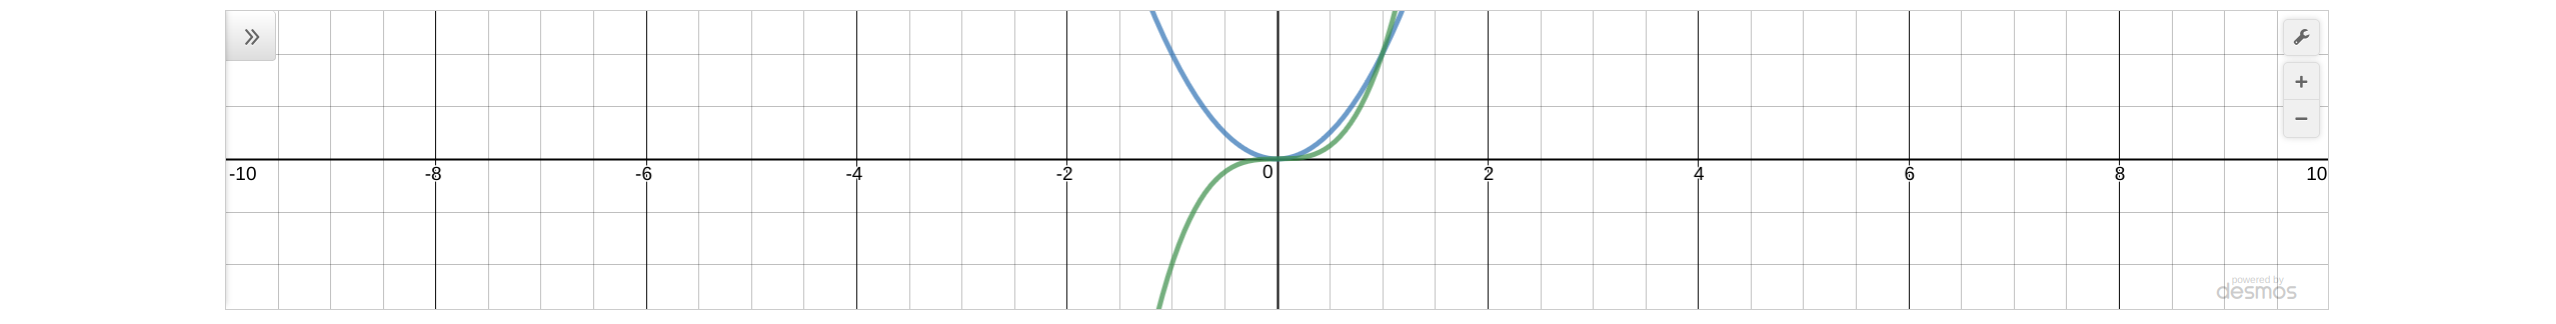
\includegraphics[width=10cm]{desmosGraph.png}
\end{image}
There are a number of options concerning the function being graphed:
\begin{verbatim}
\graph{x^2,x^3}                     %% just x^2 and x^3
                                    %%
\graph{x^2                          %%
\left\{ 1 \leq x \leq 10 \right\}}  %% restricted domain
                                    %%
\graph{\sin(x) \left\{x<0\right\},  %%
2x \left\{ x>=0 \right\} }          %% piecewise
                                    %%
\graph{r=\theta}                    %% polar 
\end{verbatim}
While the code above modifies the function being graphed, there are also several options for the display of the graph.

\paragraph{Optional arguments for \texttt{\textbackslash graph}}

\begin{description}
  \item[\tt\bfseries xmin, ymin, xmax, ymax] These set the
    size of the viewing window with
    \verb|\graph[xmin=-5,xmax=5,ymin=-5,ymax=5]{y=x^2}|.
  \item[\tt\bfseries panel] Determines if the panel is shown with
    \verb|\graph[panel]{y=x^2}|.
  \item[\tt\bfseries xAxisLabel, yAxisLabel] Gives the axes labels with
    \verb|\graph[xAxisLabel="time", yAxisLabel="distance"]{y=x^2}|.
  \item[\tt\bfseries hideXAxis, hideYAxis] Hides the axes with
    \verb|\graph[hideXAxis=true, hideYAxis=true]{x^2}|.
  \item[\tt\bfseries hideXAxisNumbers=true, hideYAxisNumbers=true] Hides the tick marks on
    the axes with
    \verb|\graph[hideXAxisNumbers=true, hideYAxisNumbers=true]{y=x^2}|.
  \item[\tt\bfseries polar] Shows polar grid lines with \verb|\graph[polar]{y=x^2}|.
\end{description}

\[
  \graph{x^2 \left\{ 1 \leq x \leq 10 \right\}}
  \graph{ \sin(x)\left\{x<0\right\}, 2x\left\{ x>=0 \right\} }
\]


\section{Desmos, Desmos 3D, and GeoGebra}

If you require further features from
\link[Desmos]{https://www.desmos.com/}, you can sign up for an account
and include your worksheets using the syntax \verb|\desmos{ID}{width}{height}|, where ID
is the widget ID and width and height are the dimensions (in pixels)
you want the embedded widget to have.
\begin{verbatim}
\begin{center}
\desmos{zwywds7med}{800}{600}
\end{center}
\end{verbatim}
which renders as:
\begin{center}
  \desmos{zwywds7med}{800}{600}
\end{center}

\providecommand{\desmosThreeD}[3]{}   % HACK: should be defined ???

The syntax for Desmos 3D is similar. Use \verb|\desmosThreeD{ID}{width}{height}|, where ID
is the widget ID and width and height are the dimensions (in pixels)
you want the embedded widget to have.
\begin{verbatim}
\begin{center}
\desmosThreeD{bb4exrhrl3}{800}{600}
\end{center}
\end{verbatim}
Seen here:
\begin{center}
  \desmosThreeD{bb4exrhrl3}{800}{600}
\end{center}

You can also use \link[GeoGebra]{https://www.geogebra.org/}. Embed the
widget using the syntax \verb|\geogebra{ID}{width}{height}|, where ID
is the widget ID and width and height are the dimensions (in pixels)
you want the embedded widget to have.
\begin{verbatim}
\begin{center}
\geogebra{XC3FXUdJ}{800}{600}
\end{center}
\end{verbatim}
\begin{center}
  \geogebra{XC3FXUdJ}{800}{600}%%https://www.geogebra.org/m/XC3FXUdJ
\end{center}

While we cannot get data from these sorts of interactives directly, the clever
author can ask questions that \textbf{use} the interactive to find a solution.

\end{document}
